% !TEX TS-program = pdflatex
% !TEX encoding = UTF-8 Unicode

% This is a simple template for a LaTeX document using the "article" class.
% See "book", "report", "letter" for other types of document.

%tells you if you use obsolote packages
%\RequirePackage[l2tabu,orthodox]{nag}

\documentclass[]{article}

\usepackage[utf8]{inputenc} % set input encoding (not needed with XeLaTeX)

%%% PAGE DIMENSIONS
\usepackage{geometry} % to change the page dimensions
\geometry{a4paper} % or letterpaper (US) or a5paper or....
% \geometry{margin=2in} % for example, change the margins to 2 inches all round
% \geometry{landscape} % set up the page for landscape
%   read geometry.pdf for detailed page layout information

\usepackage{graphicx} % support the \includegraphics command and options

% \usepackage[parfill]{parskip} % Activate to begin paragraphs with an empty line rather than an indent

%%% PACKAGES
\usepackage{booktabs} % for much better looking tables
\usepackage{array} % for better arrays (eg matrices) in maths
\usepackage{paralist} % very flexible & customisable lists (eg. enumerate/itemize, etc.)
\usepackage{verbatim} % adds environment for commenting out blocks of text & for better verbatim
\usepackage{subfig} % make it possible to include more than one captioned figure/table in a single float
\usepackage{microtype} %makes awesome kerning and punctuation come half way out the edge of the text
\usepackage{listings} %for code listings
\usepackage{color} %for colored syntax highligting

%%% Code listing
\definecolor{mygreen}{rgb}{0,0.6,0}
\definecolor{mygray}{rgb}{0.5,0.5,0.5}
\definecolor{mymauve}{rgb}{0.58,0,0.82}
\lstset{breaklines=true,
basicstyle=\footnotesize\ttfamily,
commentstyle=\color{mygreen},
keywordstyle=\color{blue},
numberstyle=\tiny\color{mygray},
tabsize=2,
language=c
}

% to include a file as a listing: \lstinputlisting{intio.c}
% inline listing: \begin{lstlisting}[frame=single]

%%% HEADERS & FOOTERS
\usepackage{fancyhdr} % This should be set AFTER setting up the page geometry
\pagestyle{fancy} % options: empty , plain , fancy
\renewcommand{\headrulewidth}{0pt} % customise the layout...
\lhead{}\chead{}\rhead{}
\lfoot{}\cfoot{\thepage}\rfoot{}

%%% ToC (table of contents) APPEARANCE
\usepackage[nottoc,notlof,notlot]{tocbibind} % Put the bibliography in the ToC
\usepackage[titles,subfigure]{tocloft} % Alter the style of the Table of Contents
%\renewcommand{\cftsecfont}{\rmfamily\mdseries\upshape}
%\renewcommand{\cftsecpagefont}{\rmfamily\mdseries\upshape} % No bold!
\usepackage{hyperref} % use hyperlinked ToC
\hypersetup{colorlinks=true, linkcolor=black}

%%%-------------------------------------------------------------------


\title{Title Here}
\author{Oskar Weigl - ow610\\ and \\ Ryan Savitski - rs510}
%\date{} % Activate to display a given date or no date (if empty),
         % otherwise the current date is printed 

\begin{document}
\maketitle

%\renewcommand{\abstractname}{Summary}
\begin{abstract}
	Write the abstract here
\end{abstract}

\tableofcontents
\clearpage

\section{Notch Filter} % (fold)
\label{sec:notch_filter}

\begin{figure}[htbp]
	\begin{center}
		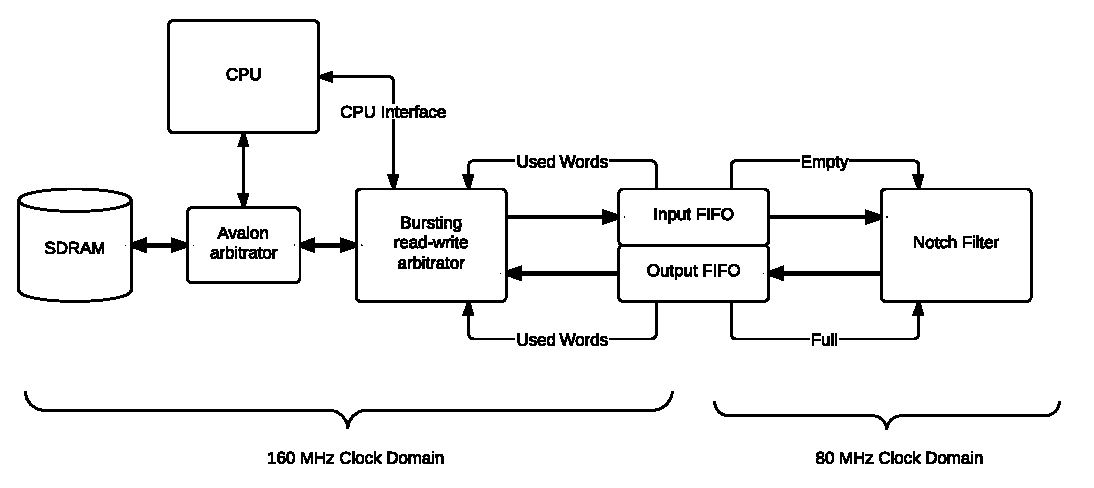
\includegraphics[width = \textwidth]{DSDNotch.pdf}
	\end{center}
	\caption{Block diagram of the Notch Filter hardware. FIFO buffers are used to allow efficient interleaved reads and writes to SDRAM. The buffers also serve as Clock Domain Crossing interfaces.}
	\label{fig:DSDNotch}
\end{figure}

\begin{figure}[htbp]
	\begin{center}
		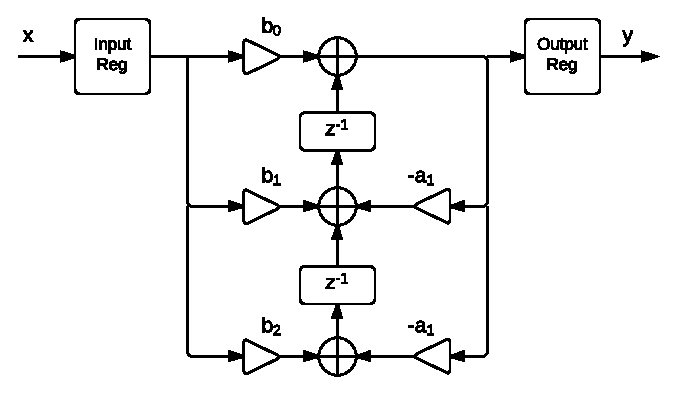
\includegraphics[width = 0.8\textwidth]{DirectFormIITransposed.pdf}
	\end{center}
	\caption{Second order Direct Form II Transposed filter architecture}
	\label{fig:df2t}
\end{figure}

\begin{figure}[htbp]
	\begin{center}
		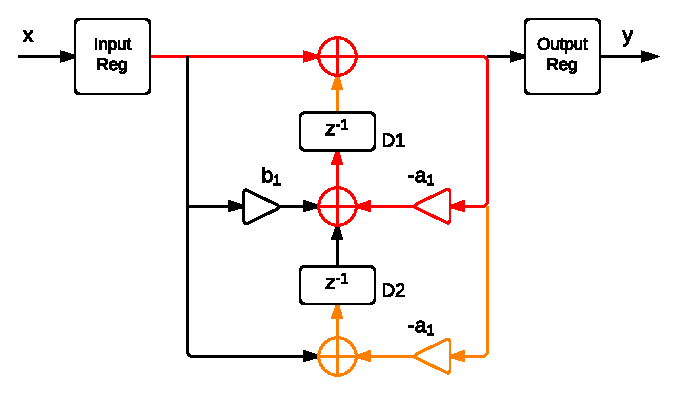
\includegraphics[width = 0.8\textwidth]{DirectFormIITransposedCritpath.pdf}
	\end{center}
	\caption{Annotated version of Figure~\ref{fig:df2t}, showing the main critical paths in the filter core. Shown in red is the path from the input register to the delay register D1. Shown in orange are the alternative paths that have almost as little slack as the red path.}
	\label{fig:df2tCritpath}
\end{figure}

architecture
implementation
performance and timing (benchmarking)
results

% section notch_filter (end)

\end{document}
